%% This is an example first chapter.  You should put chapter/appendix that you
%% write into a separate file, and add a line \include{yourfilename} to
%% main.tex, where `yourfilename.tex' is the name of the chapter/appendix file.
%% You can process specific files by typing their names in at the 
%% \files=
%% prompt when you run the file main.tex through LaTeX.
\chapter{Related Work}\label{Chap:RelatedWork}

This chapter presents the background and related work that precedes this research. These concepts lay out the foundation on which the rest of this research is conducted.

% TODO: Maybe explain what external observation and internal observation are
\section{Hardware Authenticators for \newline Two-Factor Authentication}\label{Sec:HardwareAuthenticators_2FA}

The state of the art for using hardware devices for website authentication is two-factor authentication. These devices such as the YubiKey \cite{yubico-products} resemble a small USB key which stores a private key on device. Websites that support two-factor authentication simply request the secondary mode of authentication during login. Two-factor authentication solves the security problems for login quite well \cite{questRemovePasswords}. Depending on the implementation of the specific hardware device, most provide strong resilience to targeted impersonation, physical observation, internal observation, leakage of data secrets and relying on a trusted third-party. However, as explained previously, these benefits do not pertain beyond the login point of a website and assume a lenient threat model. The adversary with control over the web-browser could simply wait for the user to faithfully log in and then launch their planned attack. 

%% 
%% \iffalse
%% , in addition to supplying a password. 
%% \fi
%% 

A number of specifications standardize two-factor authentication so that the same hardware authenticator device may be used across platforms and web services. A popular standard is Universal 2nd Factor (U2F) \cite{fido-u2f} developed by Google and Yubico, now hosted by the open-authentication industry consortium FIDO (``Fast IDentity Online'') Alliance. It is succeeded by FIDO2 \cite{fido2}, which merges WebAuthn and its extensions, including transaction authentication, into one common standard.

\section{Current Uses of Transaction Authentication}\label{Sec:CurrentUses_txAuthn}

Although transaction authentication by the WebAuthn standard is not yet commonly used, cryptocurrency hardware wallets universally support transaction authentication. The two most popular manufacturers, Ledger \cite{ledger} and Trezor \cite{trezor}, sell hardware wallets which hold the private keys and have displays. In order to send any cryptocurrency from the device, the device displays a message detailing the transaction, which the user would need to authorize on the physical device. Otherwise, the device will not sign the transaction which is required for it to proceed and be sent over the network.

In a similar but diminished vain, some banks such as Bank of America reuse two-factor authentication for sensitive or high-value monetary transactions \cite{BoA-2FA}. In order to complete the sensitive transaction, the user must redo two-factor authentication like during login. This is unlike transaction authentication in that no hardware device specific to transaction authentication is involved, and the user does not see a confirmation of the exact transaction to take place before confirming. But the process of requesting supplemental two-factor authentication on sensitive transactions aims to defend against a similar threat model as transaction authentication.

\section{Hardware Authenticators for \newline Transaction Authentication}

Hardware authenticator devices normally do not support general-purpose transaction authentication. Hardware authenticators for two-factor authentication such as the YubiKey discussed in Section~\ref{Sec:HardwareAuthenticators_2FA} do not have any display. Therefore, they are unable to perform the core function of transaction authentication, displaying a message to the user and signing it upon their confirmation. The cryptocurrency hardware wallets discussed in Section~\ref{Sec:CurrentUses_txAuthn} provide transaction authentication, but only for a limited subset of functionality relating to crypto transactions.  

%% 
\iffalse
, but none support the transaction authentication extension.

are dedicated hardware devices required by the threat model. Also, these authenticators only support regular WebAuthn two-factor authentication, not the transaction authentication extension. 
\fi
%% 

WebAuthn transaction authentication is not supported by any hardware authenticators. A few hardware authenticators and software emulated authenticators support WebAuthn, but only the regular two-factor authentication. The software emulated authenticators are intended for development and research purposes. Google has a Chrome extension that poses as a virtual hardware authenticator; it performs all of the signing in-browser \cite{virtual-authenticators-tab}. Krypton is a small company dedicated to making cryptographic authentication easy \cite{krypton}. They provide a browser plugin and phone app, which pair with one another. The plugin interfaces with the web-browser and the phone performs the cryptographic signing. 

This research must modify one of the software emulated authenticators to support transaction authentication. It uses a modified Krypton browser plugin to display the authentication message and await user consent before performing the signing also in-browser. Figure~\ref{Fig:KryptonAuthenticator} portrays the user interface of the plugin as it awaits consent before returning a signed transaction authentication object. This design deviates from the original Krypton design since it eliminates the phone app from the signing process. The security properties of the authenticator device itself is not a focus for this research. It is assumed always secure, so for prototyping and experimentation, this software modified authenticator is sufficient.

\begin{figure}[h]
  \centering
  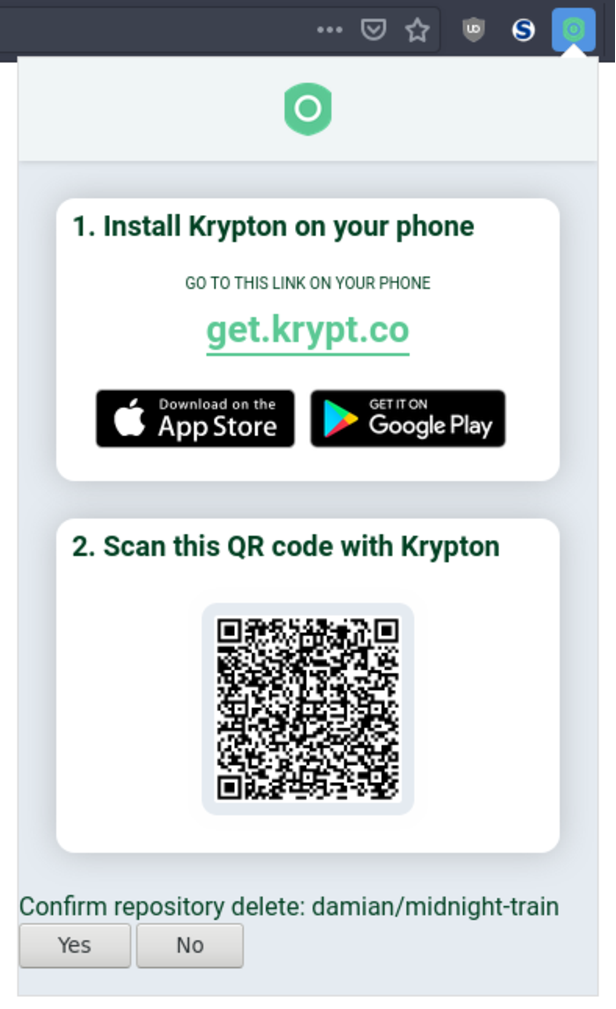
\includegraphics[width=10cm]{krypton_txauthn}
  \caption{User interface of Krypton authenticator in this thesis. It is awaiting user consent before authorizing the deletion of a repository ``damian/midnight-train''.}
  \label{Fig:KryptonAuthenticator}
\end{figure}

%% 
%% \iffalse
%% For ease of development, this research modified the Krypton browser plugin to display the authentication message and await user consent before performing the signing in-browser. It completely

%% Since the design of the hardware authenticator is not a focus for this research, it is simpler to avoid interfacing with the phone at all. 
%% \fi
%% 

\section{Web Application Firewalls}

A Web Application Firewall is a firewall that filters web traffic going to a web service \cite{web-application-firewall}. Most web application firewalls try to block malicious internet traffic from ever reaching the web-server. Common attacks defended against by web application firewalls include SQL injection, cross-site scripting and DDoS attacks. Typically, the firewall inspects incoming GET and POST request HTTP/HTTPS traffic and applies pre-configured rules to identify and filter out the undesired traffic. This thesis describes how to make a web application firewall supporting WebAuthn transaction authentication.


%% 
%% \iffalse

%% This research builds on top of the description of transaction authentication as outlined by the first version of the webauthn specification \cite{webauthn}. The webauthn specification is a comprehensive document, standardizing a protocol for two-factor authentication with configurable extensions. The protocol covers in detail how traditional two-factor authentication should be performed under webauthn as well as details how to extend it to perform transaction authentication. Transaction authentication is similar to a regular two-factor authentication event, just with some additional user involvement; the user must confirm a given transaction on a dedicated hardware device for the authentication to proceed. 

%% The purpose of transaction authentication in the eyes of the webauthn specification authors is to provide integrity to high risk operations on a website. In fact, further papers including \cite{EuroFIDO} detail use-cases of webauthn transaction authentication such as authorizing large value monetary transactions, consenting to data being shared with a third-party and authorizing a trusted service to sign a digital contract. All of these operations are very important and requesting individual authentication for each may be warranted. 

%% It appears that the state of the art for known security benefits through transaction authentication ends there. There is no research detailing how webauthn transaction authentication should be integrated into a service, what are good design choices in doing so or what the engineer should keep in mind in order to avoid accidental security holes.

%% \fi
%% 
